\documentclass{article}
\usepackage[english]{babel}
\usepackage[utf8]{inputenc}
\usepackage{amsmath,amssymb}
\usepackage{parskip}
\usepackage{graphicx}
\graphicspath{{./CS3230_images}}

\newcommand\tab[1][1cm]{\hspace*{#1}}

% Margins
\usepackage[top=2.5cm, left=3cm, right=3cm, bottom=4.0cm]{geometry}


\title{CS3230 (Analysis of Algorithms)}
\author{Jia Cheng}
\date{September 2021}

\begin{document}

\maketitle

\section{Definitions and Formula}
\paragraph{Sum of geometric progression}
\begin{align*}
	\sum_{0\leq i\leq n}r^i = \frac{r^0-r^{n+1}}{1-r}=\frac{1-r^{n+1}}{1-r}
\end{align*}

\textbf{Importantly, remember that the top term is} $1-r^{n+1}$\textbf{, not} $1-r^n$\textbf{!!!!!!}

In general, for a geometric progression $a_1, a_2, \dots, a_n$ with common ratio $r$, its sum is \begin{align*}
	\frac{a_1 - a_n\cdot r}{1-r}
\end{align*}

\paragraph{Sum of arithmetic progression}
For an arithmetic progression $a_1, a_2, \dots, a_n$ with common difference $d$, its sum is
\begin{align*}
	\frac{n\cdot (a_1+a_n)}{2}
\end{align*}

\paragraph{Decision tree} Three terms \textbf{level}, \textbf{depth}, \textbf{height}\\
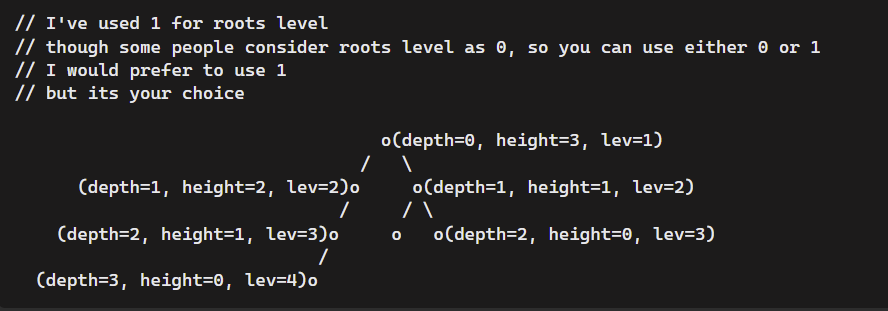
\includegraphics[scale=0.8]{tree.png}

Image from \texttt{https://stackoverflow.com/questions/63369552/depth-vs-level-of-a-tree}
\begin{itemize}
	\item For a complete binary tree, number of children at depth $k$ is $2^k$. In particular, the number of children at depth $0$ is $2^0=1$ (the root node).\\
	For example, in a comparison based sorting algorithm, the depth equals to the number of comparisons made.
	\item Height = Maximum depth of tree
	\item Level = Depth + 1
	\item Usually, depth is more useful than level since depth is $0$-indexed
\end{itemize}

\paragraph{Asymptotic notation} From wikipedia\\
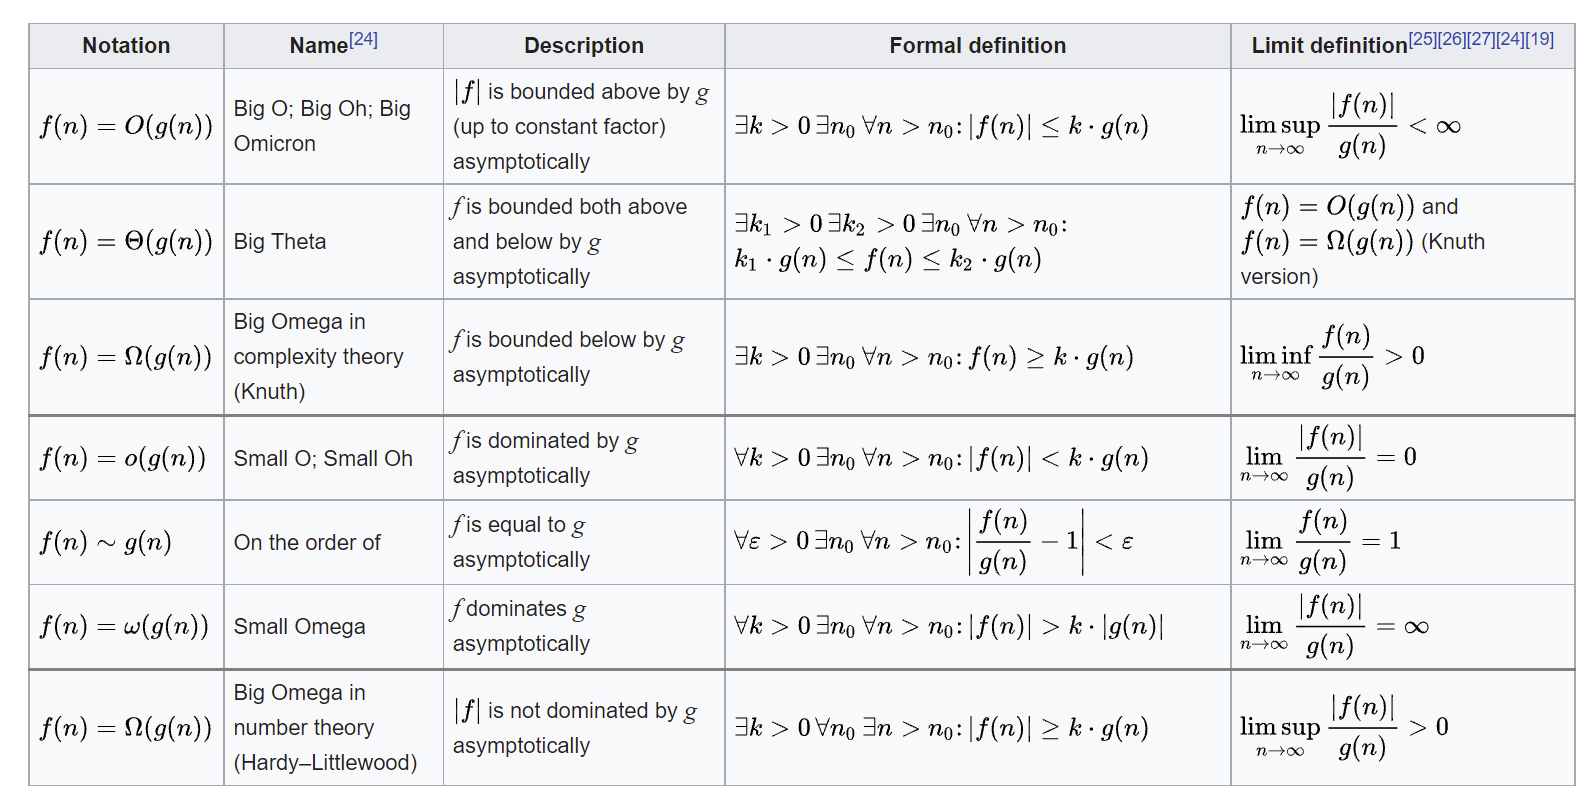
\includegraphics[scale=0.5]{asymptotic_notation.png}

\section{Bounding Techniques}
\paragraph{Integral Bound}
For a monotonically increasing function $f$,
\begin{align*}
	\int_{i-1}^j f(x)\,dx \leq \sum_{x=i}^jf(x)\leq \int_i^{j+1}f(x)\,dx
\end{align*}

\textit{Applications}
\begin{itemize}
	\item Harmonic series $H_n=\sum_{1\leq i\leq n}\frac{1}{i}\leq \int_1^{n+1}\frac{1}{i}\,di=\ln(n+1)=O(\log n)$\\
	$H_n\geq \int_1^{n}\frac{1}{i}\,di=\ln(n)=\Omega(\log n)$. Note that $\ln$ is unbounded below in $(0,1]$, so we are really using the function $g(x) = \frac{1}{x}, x\geq 1, g(x) = 0 < \frac{1}{1}, x \in [0,1]$
\end{itemize}

\paragraph{Telescoping}\mbox{}
Suppose we have the recursion $T(n) = aT(n/a) + nf(n)$. Then 
\begin{align*}
	\frac{T(n)}{n}=\frac{T(n/a)}{n/a}+f(n)
\end{align*}
and we can telescope on $S(n)=\frac{T(n)}{n}$

\paragraph{Stirling's Approximation}
\begin{align*}
	f(n)!&\sim \sqrt{2\pi f(n)}\left(\frac{f(n)}{e}\right)^{f(n)}\\
	\ln(f(n)!)&\sim f(n)\ln(f(n)) - f(n) = \Theta(f(n)\ln(f(n)))
\end{align*}


\paragraph{Logarithms}
\begin{align*}
	\lim_{n\rightarrow \infty}\frac{\log(\log(n)-k)}{\log(\log(n))} &= \lim_{x\rightarrow \infty}\frac{\ln(x-k)}{\ln(x)}\\
	&= \lim_{n\rightarrow \infty}\frac{\frac{1}{x-k}}{\frac{1}{x}}=1
\end{align*}
Hence $\log(\log(n)-k)\sim \log(\log(n))$


In general, define $f^n=f\circ f^{n-1}$, and
\begin{align*}
	\lim_{x\rightarrow \infty} \frac{\ln^n(x-k)}{\ln^n(x)} = \frac{\frac{1}{\ln^{n-1}(x-k)}\cdot\frac{1}{\ln^{n-2}(x-k)}\dots \frac{1}{\ln(x-k)}\cdot \frac{1}{x-k}}{\frac{1}{\ln^{n-1}(x)}\cdot\frac{1}{\ln^{n-2}(x)}\dots \frac{1}{\ln(x)}\cdot \frac{1}{x}}
\end{align*}
We can use strong induction to show that this limit is $1$.

\paragraph{Arithmetic sequence-like summations}
Consider a summation of the form
\begin{align*}
	\sum_{0\leq k\leq \frac{n}{m}}f(n-mk)
\end{align*}
where $m$ is a positive constant, and $f$ is a monotonically increasing function. If we expand out the summation, we realize that approximately $\frac{n}{2m}$ of the terms are greater than $\frac{n}{2}$.

To see this,
\begin{align*}
	n-mk\geq \frac{n}{2}\iff \frac{n}{2}\geq mk\iff k\leq \frac{n}{2m}
\end{align*}

Hence, we can consider the following \textbf{lower} bound
\begin{align*}
	\sum_{0\leq k\leq \frac{n}{m}}f(n-mk) \geq \sum_{0\leq k\leq \frac{n}{2m}}f(\frac{n}{2}) \approx \frac{n}{2m}\cdot f(\frac{n}{2})
\end{align*}
Usually such a bound is much tighter than simply taking the last term, $f(n)$, since we are taking into account a larger number of terms in the sum.

The no-brainer \textbf{upper} bound for such a sequence would be
\begin{align*}
	\sum_{0\leq k\leq \frac{n}{m}}f(n-mk) \leq \sum_{0\leq k\leq \frac{n}{m}}f(n)\approx \frac{n}{m}f(n) 
\end{align*}

\paragraph{Decision Tree}
The degree of branching that a decision tree based algorithm allows depends on the number of outcomes per step.\\
To be precise, suppose each step of an algorithm is able to partition the set of valid inputs into $k$ disjoint sets. Then we can think of this as branching factor $k$.

For e.g. if a single step in an algorithm allows 3 different types of outcomes, then the decision tree is ternary.

Suppose we can have $n$ possible results in total.\\
A decision tree with branching factor $k$ and height (maximum depth) $h$ has the following properties. Let $L$ be the number of leaves of the tree.
\begin{itemize}
	\item The leaves represent the outcomes. $L\leq 2^h$. Equality holds when the tree is complete.\\
	Example: A comparison based sorting algorithm has a branching factor of 2. Hence if $h$ comparisons are made, the tree has at most $2^h$ leaves. A necessary condition for the sorting algorithm to be correct (when there are $n$ elements) is that $L\geq n!$. Hence $2^h\geq n!$ and we have the familiar bound $h\geq \lg n!$
	\item The height of the tree represents the number of operations/"steps" that are taken. E.g. When $0$ operations are taken, the tree is of height $0$ and it only consists of $1$ leaf which is also the root node. Hence there are $2^0 = 1$ leaves.
\end{itemize}

When are decision trees ineffective in analysis?
\begin{itemize}
	\item Decision trees are good when \textbf{distinct inputs give distinct answers}. In other words, a correct algorithm is necessarily injective. Due to this property, if a decision tree is unable to produce as many leaves as the possible range of inputs, i.e. at least 1 leaf encompasses $>1$ input, then \textbf{the algorithm is unable to distinguish 2 distinct inputs with distinct solutions} and hence must be incorrect. 
	\item An example of incorrect usage of decision tree would be a simple query model problem. Taken from lecture 1,\\
	\textit{In the string query model, the input is a string of n bits. In one time unit, an algorithm can query one bit of the string. All other operations on the string can be performed at 0 cost. Let Zero be the problem of deciding whether an input string x is the all-zero string or not. The optimal algorithm for Zero has query complexity n.}\\
	There are $2^n$ valid inputs, since each entry $A[i]$ of an array $A$ can either be $1$ or $0$. Additionally, the decision tree is a binary one, since when the algo queries index $i\in \{1,\dots,n\}$, we either reply $A[i]=1$ or $A[i]=0$.\\
	However, even if the height of the decision tree is strictly less than $n$, such that there are strictly fewer than $2^n$ leaves, \textbf{we cannot immediately claim that the algo is incorrect}. Because it is certainly possible that the input $A[1]=A[2]=\dots=A[n]=0$ is in its own leaf, alone. The other leaves that encompass multiple inputs then all give the same answer (i.e. the string is not the All-Zero string). Then the adversarial argument would not work here.
\end{itemize}


\paragraph{Jensen's inequality for expected values}\mbox{}

Let $X$ be a random variable and let $f$ be a function.\\
If $f$ is concave (e.g. $x\mapsto \sqrt{x}$), then $E[f(X)]\leq f(E[X])$ (e.g. $E[\sqrt{X}]\leq \sqrt{E[X]}$) .\\
If $f$ is convex (e.g. $x\mapsto x^2$), then $E[f(X)]\geq f(E[X])$.\\
It is due to the convexity of the square function that $Var(X) = E[X^2]-E[X]^2\geq 0$


\section{Distributions}
\paragraph{Poisson approximation of Binomial Distribution}
Given binomially distributed $X\sim B(n, p)$, $X\approx Y\sim Poi(\lambda = np)$, where $Y\in \{0,1,2,\dots\}$

\begin{center}
	p.m.f. of $Y$: $P(Y=k) = e^{-\lambda}\frac{\lambda^k}{k!}$\\
	$P(Y=0) = \exp(-\lambda)$\\
	$P(X>0) \approx P(Y>0) = 1 - \exp(-\lambda)$
\end{center}


\section{Graphs}
Suppose a graph has vertices $V$ and edges $E$. Some common concepts associated with graphs (which we can use to argue or prove things are:
\begin{itemize}
	\item $V$
	\item Pairs of points ($V$ choose 2), adjacency matrix
	\item $E$
	\item Degree of vertex $v$, $deg(v)$
	\item Endpoints of edges
	\item Coloring nodes (this is a more general concept, and colors can often mean different things in different contexts)
\end{itemize}

\paragraph{Handshake Lemma}
\begin{align*}
	\sum_{1\leq i\leq |V|}deg(v_i) = 2\cdot |E|
\end{align*}

\section{Algorithms}
Themes

\paragraph{Similar subroutines to well-known algorithms}
\begin{itemize}
	\item Quickselect
	\item Partition
	\item Merge
	\item Radix sort (e.g. when items to sort, usually integers, are bounded above)
	\item Linear search
	\item Binary search (e.g. Searching the maximal element in a sorted, then cyclically rotated array)
\end{itemize}

\paragraph{Paradigms}
\begin{itemize}
	\item Divide and conquer
	\begin{itemize}
		\item Returning additional metadata (to improve asymptotic efficiency) e.g. O(n) version of maximal contiguous subarray sum/product
	\end{itemize}
	\item Streaming (e.g. find majority element)
\end{itemize}


\subsection{Dynamic Programming}
\paragraph{Subproblem Graph} CLRS Pg 367, 380-381

Looking at the graph, the runtime of a memoized algorithm is the number of directed edges. (Notice that each edge is "traversed" exactly once). Hence, by summing the outdegrees of each vertex, we can obtain the overall runtime.


The edges represent calling the subprocedures, but not "stepping into" them.\\
The outdegree of a vertex is usually (but not always) the runtime of a single call to the procedure without further recursion. \\
If the procedure itself has something additional computation involved internally, then we will also need to factor this into the runtime. This can be represented by the vertex itself.\\
Combining the above 2 points, we need to add up the edges and the vertices.

Hence the runtime of a memoized procedure, say $func$ is $T(n) = O(\sum_{1\leq i\leq n}S(i))$, where $S(i)$ is the runtime of a call to $func(i)$ without going into the recursive calls.

\paragraph{A loose upper bound} Adapted from CLRS Pg 380
There are 2 factors that determine the running time of a DP solution
\begin{itemize}
	\item (1) how many subproblems an optimal solution to the original problem uses,
	\item (2) how many choices we have in determining which subproblem(s) to use in an
optimal solution
\end{itemize}

A (possibly loose) upper bound for the DP solution would then be the product of (1) and (2).

\end{document}


